\documentclass[12pt,a4paper,oneside,openany]{memoir} 
% Skabelon af DTU's LaTeX support gruppe, v20090423

\usepackage[utf8]{inputenc} 
%\usepackage[danish]{babel} % danske overskrifter
\usepackage[T1]{fontenc}   % fonte (output)
\usepackage{lmodern}       % vektor fonte
\usepackage{fancybox, graphicx}      % indsættelse af billeder
\usepackage{palatino}      % lækker font
\usepackage{pdfpages}      % pdf som forside evt
\usepackage{todonotes}
\usepackage{microtype}
% \linespread{1.3}           % kræver lidt mere line spacing
\usepackage{multirow}

\newcommand{\code}[1]{\texttt{#1}}
\newcommand{\HRule}{\rule{\linewidth}{0.5mm}}

%\addto\captionsdanish{
%  \renewcommand{\contentsname}%
%    {Indholdsfortegnelse}     %
%} % Så bruger vi bare 'Indholdsfortegnelse' i stedet for 'Indhold'


\usepackage{underscore}
\usepackage{pdflscape}
\usepackage{todonotes}

\usepackage[plainpages=false,pdfpagelabels,pageanchor=false]{hyperref} % aktive links
\hypersetup{
    pdfborder = {0 0 0}
}
\def\sectionautorefname{afsnit}

\usepackage{memhfixc}  % rettelser til hyperref

\usepackage{tipa}
\pretolerance=2500     % højt tal, mindre orddeling og mere space mellem ord.
% 3000 er okey, 1000 er for lidt, 5000 i overkanten, 8000 er for meget..

\usepackage[font=small,labelfont=bf,labelsep=endash]{caption}
 
\pagestyle{headings}


\makechapterstyle{mortenovi}{%
\setlength{\beforechapskip}{0cm}%længde fra top af side til kapitel-overskrifter
\setlength{\afterchapskip}{1cm}%længde fra kapiteltekst til body-tekst
\setlength{\midchapskip}{2cm}%længe mellem kapitelnummer og kapiteltekst
\renewcommand\chapnamefont{\normalfont\Large\scshape\raggedleft}
\renewcommand\chaptitlefont{\normalfont\Huge\bfseries\sffamily}
\renewcommand\chapternamenum{}%default "kapitel"
\renewcommand\printchapternum{%
    \makebox[0pt][l]{%
    \hspace{0.4em}
    \resizebox{!}{4ex}{\chapnamefont\bfseries\sffamily\thechapter}}
    }%"kapitel. x"-linjen og dens boxe og bredder - prøv at sætte xyz ind først på de tre linjer respektivt.
\renewcommand\afterchapternum{\par\hspace{1.5cm}\hrule\vspace{0.5cm}}
\renewcommand\afterchaptertitle{\vskip\onelineskip \hrule\vskip\afterchapskip
}}
\chapterstyle{mortenovi}

\maxtocdepth{subsection} %Only parts, chapters and sections in the table of contents
\settocdepth{subsection}

% \includeonly{forord,testing} % Kompiler kun de kapitler du arbejder med.

\usepackage{listings}
\usepackage{color}

\renewcommand*\lstlistingname{Kode}

%for diagbox
\usepackage{diagbox}
\usepackage{booktabs}
% Done

\definecolor{dkgreen}{rgb}{0,0.6,0}
\definecolor{gray}{rgb}{0.5,0.5,0.5}
\definecolor{mauve}{rgb}{0.58,0,0.82}

\lstset{frame=tb, %lr
  language=Java,
  aboveskip=3mm,
  belowskip=3mm,
  showstringspaces=false,
  columns=flexible,
  basicstyle={\small\ttfamily},
  numbers=none,
  numberstyle=\tiny\color{gray},
  keywordstyle=\color{blue},
  commentstyle=\color{dkgreen},
  stringstyle=\color{mauve},
  breaklines=true,
  breakatwhitespace=true,
  basicstyle=\tiny\ttfamily
}

\usepackage{cleveref}


\begin{document}
%\includepdf[fitpaper]{billeder/forside}


\begin{center}
\thispagestyle{empty}

% Upper part of the page. The '~' is needed because \\
% only works if a paragraph has started.

\textsc{\LARGE IT University of Copenhagen}\\[1.5cm]

\textsc{\Large Second Year Project: \\ Software Development in Large Teams with International Collaboration}\\[0.5cm]

% Title
\HRule \\[0.4cm]
{ \huge \bfseries Pre-handin 
    %\large \\ [0.4cm] 
    }

\HRule \\[1cm]


% Author and supervisor
\begin{minipage}{1\textwidth}
\begin{center} \large
Adam William Engsig \\
Anders Fischer-Nielsen \\
Anders Wind Steffensen \\
Cecilie Strunge Jensen \\
Mikael Lindemann Jepsen\\
Morten Albertsen
\end{center}
\end{minipage}


\vfill

% Bottom of the page
{\large \today}

\end{center}

\frontmatter%

%\include{abastract}
%\include{preface}

%\tableofcontents* % stjernen betyder vi ikke har den med i vores indholdsfortegnelse

\tableofcontents

\newpage

\mainmatter%

%input chapters here

\chapter{Introduction}\label{introduction}

This report describes the software, that was designed and built by the
group during the project in \emph{Second Year Project: Software
Development in Large Teams with International Collaboration}.

As a brief introduction, the purpose of the system is to construct a
generic workflow system, that enables users to get an overview of and
execute the events within a workflow through a Windows client. An event
is here a part / step of a workflow.

The project hence is concerned with implementing the software within the
Windows client, the events and a central server, that acts an
intermedryte between the client and the events. The three parts must be
implemented such that they run in a distributed fashion.

\chapter{Implemented workflow}\label{implemented-workflow}

This section describes the workflow, that was implemented as a sample workflow. The workflow was based at a textual description, provided by our external partner in Brazil.

The workflow concerns medical care and treatment at a hospital.

We have deliberately decided to simplify and omit certain parts of the
given workflow. This was done, so the group could focus at implementing
core-functionality first, before moving on to more complex workflows.
The system should be able to handle more complex workflows than the one
presented, but has not been tested thorougly enough at the moment. The
group hopes to be able to guarantee support of more complex workflows in
the second part of this project.

The workflow, that is implemented in the delivered software, is seen in Figure \ref{fig:WorkflowIllustrationFromDCRGraphs} in 
Appendix, and generated through the online-tool available
at \href{www.dcrgraph.net}{DCRGraph.net}

\chapter{How to run the system}\label{how-to-run-the-system}

This section describes how to run the provided software; namely the
Windows Client ("Client'')

In order to start up the Client, double-click on the Client.exe-file
(supplied in handin-folder) with the Flow-icon.

\section{The user-interface}\label{the-user-interface}

The first window that is shown is the Login-window (see picture
below)\\
In this windows type in your username and click on the
Login-button.

For username, either
\begin{itemize}
\item Log in as \textit{Admin} This will allow you to execute any event within the workflow
\item Use a role (as seen on the DCRGraph). For instance, to execute PatientCheckIn as CheckInReceptionist, log in as \textit{CheckInReceptionist}. Recall, that you must have the correct role to execute an event. 
\end{itemize}



\begin{figure}[h]
\centering
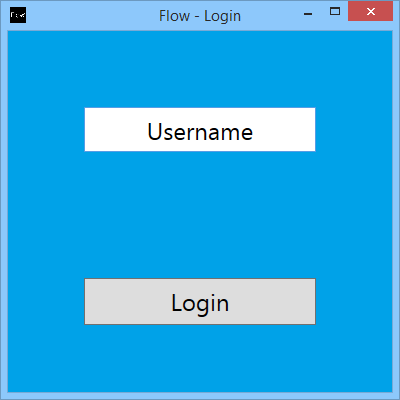
\includegraphics[width=0.8\textwidth]{ClientLogin.png}
\caption{Client Login Window}
\end{figure}


If the username is correct and corresponds to a user on the
Workflow-Server the login will succeed and the user will be presented
with a new window which is the main Flow window.

\begin{figure}[h]
\centering
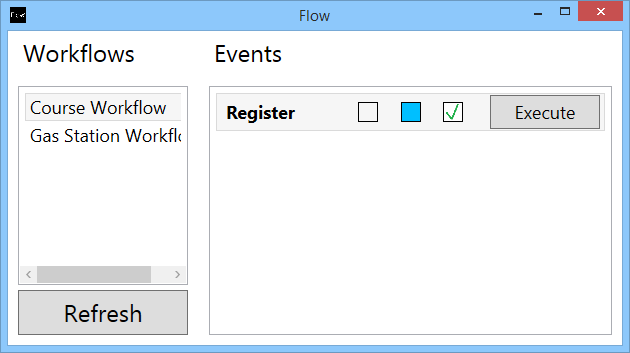
\includegraphics[width=0.8\textwidth]{ClientMainView.png}
\caption{Client Main Window}
\end{figure}

In the main Flow window, the user is presented with a list of workflows
to the left. If nothing is shown, and the user is sure that a workflow
should be present, the Refresh-button can be pressed.

The Refresh-button is also used to see changes in workflows, so if the
Workflow-Server is updated with a new workflow, the user must press
Refresh to see the new content.

To Reset a workflow to it's initial state, press the Reset button.

When a workflow is selected (in the left pane), the right part of the
window is updated. This part of the window shows the events of the
current workflow.

The information shown is collected from the Event-server itself, so some
information might take a while to receive. When the title of the Event
is shown, the Event has been loaded.

For every event a title is shown (Register in picture above), a few
status-boxes (described below) and an Execute-button.

The title is the user's way of identifying the Event. There is no rules
about naming of the Events, so two Events could in theory have the same
name. We do not encourage it though.

The three status-boxes represents the state of the given Event; from
left to rigt: Pending, Included and Executed.

The Pending-box has a red exclamation-mark when the Event is Pending. An
Event is Pending if another Event has marked it as such when executed.
This means that this is the expected action to take when the other Event
has been fulfilled. An Event is Pending until it has been either
executed or excluded.

The Included-box is blue whenever the Event is included. An Event can be
included which means that it is currently possible to execute the Event
when all of its conditions has been fulfilled. It can also be excluded
which means it is not possible to execute the Event until another action
makes it included again.

The Executed-box is checked if an Event has been executed at least once
for this workflow.

The Execute-button tells the Event to execute, which effectively means
that it marks itself as executed (if possible) and tells all of its
neighboring Events to update their state according to the rules of the
workflow.

The button is active only if the Event is currently executable, which
means it must be included and all of its conditions must be executed at
least once.

\section{Settings file}\label{settings-file}

The client creates a settings file (located at ????), where a few
informations are saved.

It is possible to use the settings file to change the URL of the
Workflow-Server, which means it is possible to point the client to a
different Workflow-Server if desired.

The settings file also remembers the username of the last successful
login, so the user can login without writing the username every time.

\chapter{System architecture}\label{system-architecture}

This section provides a birds-eye view of how the system was implemented
and what parts is was broken down into.

To fulfill the requirements of the project, three subsystems are
created: a central server (``Server''), a client (``Client) and events
(''Event``). The three subsystems are described in the following
section.

\section{Central Server}\label{central-server}

The central Server functions as a RESTful WebAPI, where Events can hook
up onto an existing workflow and the client can retrieve a list of
workflows and related events. The server subsystem is implemented in C\#
using the ASP.NET Web API framework.

\section{Client}\label{client}

The main functionality of the client subsystem is to provide the users
an overview of workflows and events on the workflows, and provide the
user with a way to send an Execute call to a specific event. The Client
is implemented in C\# using the .NET framework WPF for GUI components.
The client has a connection submodule which handles all outgoing calls
to both the server and events.

\section{Event}\label{event}

The event subsystem is implemented in C\# using the ASP.NET Web API
framework, which allows for easy routing and setup of a RESTful WebAPI.
An event also have submodules which controls all outgoing calls to the
server and to the events which (the event) is related to. The
implementation of an event allows for multiple events to be stored at
either, the same machine or be distributed across network and multiple
machines or a combination of the two.

\chapter{Testing}\label{testing}

This section describes how the group has tested the system and includes
a discussion of to what extent we believe the software works as
intended.

A variety of testing approaches have been used to test the system during
development. These include unit-, integration-, system- and acceptance
testing in varying degrees. Acceptance testing has also been applied
after the inital tests were developed.

\section{Unit Testing}\label{unit-testing}

The major components handling data that have been developed by the team
(not Microsoft's libraries) have been unit-tested to ensure that their
functionality was correct.

The unit-tests can be found and run within the provided Visual
Studio-solution in a project following the naming-convention:

\[<TargetProject>.tests\]

for instance the project \emph{Server.tests} contains the unit-tests of
Server.

\subsection{Server}\label{server}

The unittests on Server are found in the Server.tests project (in the
provided Visual Studio solution)

The WebAPI controller and server logic classes have been unit tested as
follows:

\subsubsection{IServerLogic}\label{iserverlogic}

ServerLogic is the implementation of the IServerLogic interface, and has
therefore been tested according to the methods specified in this
interface. Mocking has been used extensively (using the Moq NuGet
package) to ensure that the logic was tested in an isolated and
controlled environment. The logic saves data to an instance of
IServerStorage, which is mocked to enable testing. Every method in this
interface is mocked, and saves and retrieves data from an in-memory list
using callback methods.

\subsubsection{WorkflowsController}\label{workflowscontroller}

Mocking is used to test the implementation of the WorkflowController
class - again to test in a controlled environment. An IServerLogic
instance is mocked and returns a List of elements when a method is
tested. Incoming HTTP requests are handled by the WorkflowsController
and therefore methods handling GET, POST, PUT and DELETE requests have
been tested using a IServerLogic mock.

\subsection{Event}\label{event-1}

The unit-tests concerning Event are located in the Event.tests project
(in the provided Visual Studio solution)

The outgoing communicator, WebAPI controller and event logic classes
have been unit tested as follows:

\subsubsection{EventCommunicator}\label{eventcommunicator}

The EventCommunicator should throw certain expections when receiving
invalid requests. This has been tested for methods in the
IServerFromEvent interface.

\subsubsection{EventLogic}\label{eventlogic}

EventLogic is the implementation of the IEventLogic interface. The
methods in this interface have been unit tested by creating an in-memory
instance of IEventStorage and testing against this. Assertions for
expected results (including exceptions) is used to test that methods
return the expected results.

\subsubsection{EventStateController}\label{eventstatecontroller}

The locking functionality of events has been tested using unit testing
and assertions for expected results.

\subsection{Client}\label{client-1}

The unittests on the client are located in Client.tests projects (in the
provided Visual Studio-solution).

The connection from the client to the server has been unit tested as
follows:

\subsubsection{ServerConnection}\label{serverconnection}

The ServerConnection inherits from the IServerConnection interface and
the methods defined in this interface have been unit tested. An instance
of HTTPClientToolbox is mocked to ensure that the ServerConnection can
be tested in an isolated environment. Testing that the correct
exceptions are thrown on invalid requests and correct data is returned
on valid requests is done by assertion.

\section{Integration Testing}\label{integration-testing}

Formal test cases have been specified, but have not been evaluated
formally. Most functionality has been tested throughout development, but
test results have not been written down due to time pressure. Getting
the system to "just work'' after unit testing was completed, has been
main focus for the team.

\section{System Testing}\label{system-testing}

System testing has not yet been formally completed.

\section{Acceptance Testing}\label{acceptance-testing}

Acceptance testing would preferrably be done by the receiver/user of the
system using test cases specified either by the client or the
developers. Acceptance testing has not been done yet, as this was first
planned to be carried out following this pre-handin.

\section{Discussion of
testing-approach}\label{discussion-of-testing-approach}

The team's testing approach has mainly been centered around
unit-testing.

It has not been able to carry out acceptance-testing with external
partners as of yet.

The group's confidence in the system is currently restricted to a
per-module level due to time-pressure. Integration testing and system
testing should be completed before handing in part 2 of the system.

\chapter{Conclusion}\label{conclusion}

The delivered software at this point provides a starting-point for the project's
second part. We think the project is ambitious, and getting the features right will be a focus for the project's second part. 

\chapter{Questions regarding workflow in Brazil}\label{questions-regarding-workflow-in-brazil}

\begin{itemize}
\itemsep1pt\parskip0pt\parsep0pt
\item
  In 7) the provided workflow-description, who's responsible for
  ``\emph{prepare patient}''?
\item
  ``\emph{The physician may recommend the patient an appointment with a
  specialist or request some exams}'' Will the one exclude the other, or
  could both happen, i.e. could the physician both recommend the patient
  an appointment \textbf{and} request some exams?
\item
  In 9) a patient can be referred to ROTA. Sould the hospital charge the
  government after referal or not?
\item
  In connection to ROTA. Can an examinator refer a patient to ROTA?
\end{itemize}

\chapter*{Appendix}

\begin{figure}[h]
\centering
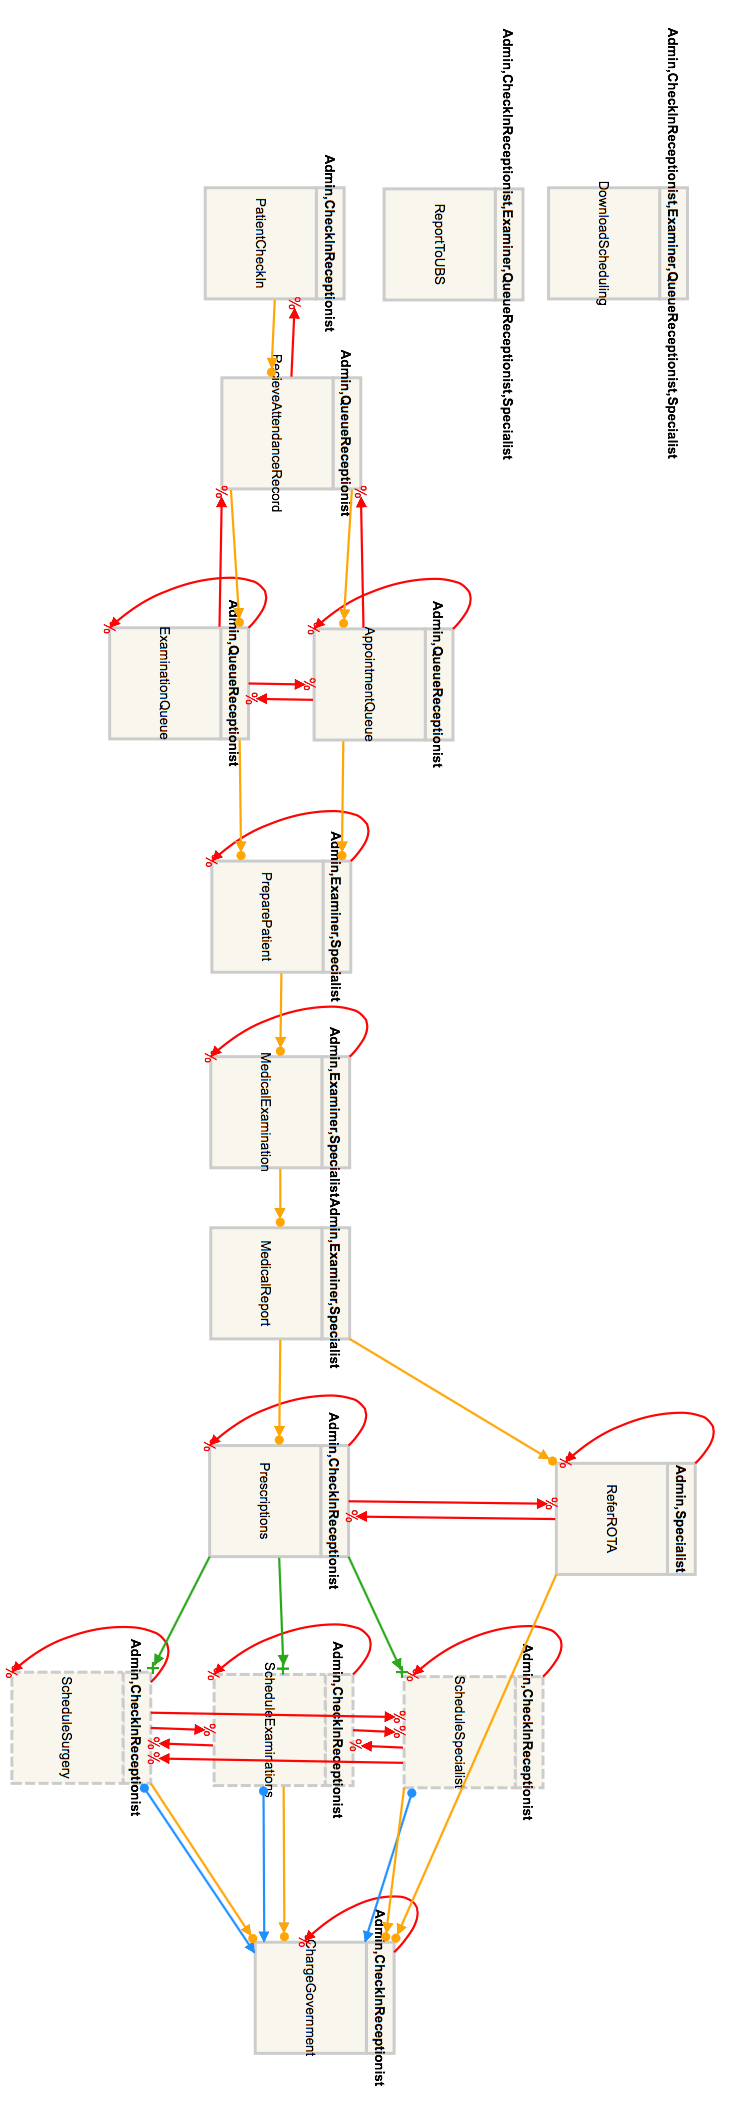
\includegraphics[width=0.45\linewidth]{Workflow.png}
\caption{Implemented workflow in delivered software. Workflow represents healthcare-workflow from provided description. In PDF, zoom in to getter view \label{fig:WorkflowIllustrationFromDCRGraphs}}
\end{figure}



\end{document}